%% ============================================================================
%% Planetary Wave Forcing Suppresses Natural Dry Slab Avalanche Activity
%% via Stratospheric Sudden Warmings
%%
%% Target: Nature Geoscience (Article format)
%% Format: Nature Portfolio Design Template
%% ============================================================================
\newif\ifdramaticfigures
\dramaticfiguresfalse  % Default: use original figures

\documentclass[11pt,letterpaper]{article}

% Packages
\usepackage[utf8]{inputenc}
\usepackage[T1]{fontenc}
\usepackage{amsmath,amssymb}
\usepackage{graphicx}
\usepackage{booktabs}
\usepackage{hyperref}
\usepackage[numbers,sort&compress]{natbib}
\usepackage{xcolor}
\usepackage{geometry}
\usepackage{lineno}
\usepackage{tcolorbox}
\usepackage{adjustbox}    % For table width adjustment
\usepackage{array}        % Enhanced column types
\usepackage{tabularx}     % Auto-width tables
\usepackage{makecell}     % Multi-line cells
\usepackage{multirow}     % Multi-row cells

% Define glossary box style
\newtcolorbox{glossarybox}[1][]{
  colback=gray!5,
  colframe=gray!50,
  fonttitle=\bfseries,
  title=Glossary of Abbreviations,
  #1
}
\usepackage{caption}
\captionsetup{font=small,labelfont=bf}
\usepackage{setspace}
\onehalfspacing
\usepackage{tikz}
\usetikzlibrary{arrows.meta,positioning}

% Nature formatting
\geometry{margin=1in}
\linenumbers
\sloppy  % Allow more flexible line breaking to prevent overfull hboxes

% URL formatting - allow breaks at more characters
\makeatletter
\g@addto@macro{\UrlBreaks}{\UrlOrds}
\makeatother

% ---- Title ----
\title{\textbf{Planetary Wave Forcing Suppresses Natural Dry Slab Avalanche Activity via Stratospheric Sudden Warmings:\\
Multi-Country Evidence, Process-Model Validation, and Count--Rating Dissociation}}

\author{
    Abduxoliq Ashuraliyev$^{1,*}$
    \\[6pt]
    $^1$Independent Researcher, Tashkent, Uzbekistan\\[6pt]
    $^*$Corresponding author: Jack00040008@outlook.com\\[6pt]
    ORCID: 0009-0003-5482-5526
}

\date{}

\begin{document}
\maketitle
\thispagestyle{empty}

% ============================================================
%  ABSTRACT  (~200 words)
% ============================================================
\begin{abstract}
Stratospheric sudden warming (SSW) events produce persistent surface weather anomalies, yet their consequences for geophysical hazards remain unexplored.
Here we identify a previously unknown connection: SSW episodes drive a large, reproducible reduction in natural dry slab avalanche activity across four countries and two continents, mediated by a ``threshold amplification'' mechanism in which modest stratospheric-origin weather shifts produce disproportionately large hazard responses by switching binary trigger conditions across mountain networks.
In Switzerland (21~winters, 16~SSW events), 14 of 16 events show reduced counts (geometric mean rate ratio $\mathrm{RR} = 0.32$; 95\% CI $[0.20, 0.54]$; $d = -1.06$).
Norwegian avalanche danger levels decrease concordantly ($d = -0.67$; $P < 10^{-6}$), and all four Utah SSW events show decreased counts ($\mathrm{RR} = 0.34$).
A specification curve of 180 analytical variants confirms robustness: 100\% show $\mathrm{RR} < 1$ (permutation $P < 0.001$).
Five-country EAWS data reveal a predictable geographic gradient in hazard response ($r = 0.69$, $P = 0.0004$), confirmed out-of-sample by independent ALBINA bulletin data---demonstrating that the spatial structure of SSW--surface coupling is systematic, not stochastic.
A count--rating dissociation---danger \emph{ratings} increase while occurrence \emph{counts} decrease---and a differential trigger response---human-triggered avalanches increase ($\mathrm{RR} = 1.81\times$ relative to natural) while natural triggers are suppressed---reveal a ``loaded gun'' mechanism: SSW-associated cold regimes suppress surface-energy triggers ($-57\%$ warming, $-29\%$ rain) while preserving snowpack instability.
Hemispheric verification via Aura/MLS stratospheric chemistry, SNOTEL surface observations, and Northern Hemisphere snow cover ($d = +1.13$) confirms that every link in the mechanism chain is independently significant.
The temporal profile---suppression emerging before SSW onset---identifies planetary wave forcing as the common cause rather than top-down stratospheric forcing.
\end{abstract}

\noindent\textbf{Plain Language Summary.}
Snow avalanches in the Alps kill hundreds of people each year. We discovered that a dramatic atmospheric event called a ``stratospheric sudden warming''---where temperatures 30--50~km above Earth surge by 30--40~°C in just a few days---is consistently followed by a sharp drop in natural avalanche activity at the surface. Across 16 such events in Switzerland over 21~winters, natural dry slab avalanches decreased by 68\% on average. The same pattern appears in Norway and Utah using entirely different measurement systems. Using output from SNOWPACK, a physics-based snowpack model run at 130~Swiss stations, we find that the snowpack actually becomes \emph{less} stable during these events---but the natural triggers that would normally release avalanches (surface warming, rain-on-snow, solar radiation) are simultaneously suppressed by the cold regime. This creates a ``loaded gun'' situation: a primed snowpack without natural release, which may explain why human-triggered avalanche rates increase during these windows. Because stratospheric sudden warmings can be predicted 1--2~weeks in advance, our findings could extend avalanche hazard forecasting beyond the current 5--7~day weather-based window.

% ============================================================
%  INTRODUCTION
% ============================================================
\section*{Introduction}

Stratospheric sudden warming events are among the most dramatic circulation phenomena in the middle atmosphere. During an SSW, the wintertime stratospheric polar vortex weakens or reverses, with zonal-mean temperatures at 10~hPa increasing by 20--40~K within days\cite{Matsuno1971,Charlton2007}. The downward coupling of SSW signals to the troposphere is well established: SSW events precede persistent surface weather anomalies including cold-air outbreaks over Eurasia and North America, shifts in the North Atlantic Oscillation (NAO) toward its negative phase, and altered precipitation patterns across mid-latitudes\cite{Baldwin2001,Thompson2002,Kidston2015}. These tropospheric responses typically emerge 1--4~weeks after SSW onset and can persist for 30--60~days\cite{Sigmond2013}.

Crucially, SSW events are themselves \emph{caused} by enhanced tropospheric planetary wave activity that propagates upward and breaks in the stratosphere\cite{Matsuno1971,Polvani2004}. Any surface anomaly observed around SSW onset could therefore reflect either top-down stratospheric forcing (SSW~$\to$~troposphere~$\to$~surface) or a common-cause pathway in which the same planetary wave forcing simultaneously triggers the SSW and reorganises surface weather. Distinguishing these interpretations requires careful attention to the temporal profile, dose--response relationships, and mediation pathways.

Despite the established influence of SSW events on surface weather, their consequences for geophysical hazards have never been systematically quantified---a striking gap given that threshold-dependent processes (avalanches, landslides, floods) should amplify modest atmospheric anomalies into disproportionate hazard changes. Snow avalanches---responsible for approximately 250~fatalities per year worldwide\cite{Techel2016}---are fundamentally sensitive to the meteorological variables that SSW events perturb: temperature, precipitation, wind speed, and their temporal gradients\cite{Schweizer2003,Schweizer2008}. Dry slab avalanches, in particular, are triggered when the shear stress on a buried weak layer exceeds its strength---a threshold process governed by snow loading rates, temperature metamorphism, and radiative balance\cite{McClung2006,Reuter2018}.

Here we present, to our knowledge, the first quantitative evidence that stratospheric variability measurably affects a surface geophysical hazard: a large, reproducible reduction in natural dry slab avalanche activity during SSW windows across three countries using independent measurement systems. We quantify the effect using rate ratios relative to day-of-year-matched controls, test candidate mechanisms through ERA5 reanalysis composites, verify snowpack stability changes with independent Rutschblock field tests, and probe annular-mode mediation. We report all results transparently, including null findings for mechanistic pathways, and apply Benjamini--Hochberg false discovery rate correction across all primary hypothesis tests.

% ============================================================
%  RESULTS
% ============================================================
\section*{Results}

\subsection*{SSW events suppress natural dry slab avalanches in Switzerland}

We analysed daily counts of natural-trigger dry slab avalanches (size class $\geq$1) from the Swiss WSL/SLF database spanning 21~winters (1998/99--2018/19; 7,518~days). This variable isolates weather-driven release events by excluding human-triggered avalanches, which depend on recreational exposure patterns rather than atmospheric forcing.

For each of 16~SSW events identified from the Butler et al.\ catalog\cite{Butler2015}, we computed observed counts in a $\pm$15-day window around onset and compared them to expected counts derived from day-of-year-matched climatology ($\pm$3~days, non-SSW winters only). The rate ratio $\mathrm{RR} = \mathrm{observed} / \mathrm{expected}$ measures the multiplicative change in avalanche activity.

Of 16~SSW events, 14 show $\mathrm{RR} < 1$ (sign test $P = 0.002$; Fig.~\ref{fig:ssw_matched}). The geometric mean $\mathrm{RR} = 0.32$ (95\% bootstrap CI: $[0.20, 0.54]$), corresponding to a 68\% reduction in natural dry slab counts. The effect is highly significant across multiple test frameworks: paired $t$-test on $\log(\mathrm{RR})$, $P < 0.001$; Wilcoxon signed-rank, $P < 0.001$; permutation test (10,000 iterations), $P = 0.0005$. Cohen's $d = -1.06$ indicates a large effect size.

The two exceptions are February 2018 ($\mathrm{RR} = 1.05$; the split-vortex ``Beast from the East'' that produced an extreme cold-air outbreak over western Europe, generating exceptional wind slab loading on exposed aspects---a synoptic pattern that \emph{enhanced} rather than suppressed natural triggers) and January 2019 ($\mathrm{RR} = 3.43$; this SSW coincided with the heaviest Alpine snowfall episode since 1999, which deposited extreme loading that overwhelmed trigger-suppression effects---the only event where cumulative precipitation exceeded $3\sigma$ above the DOY mean). Leave-one-out cross-validation confirms robustness: all 16 jackknife folds retain $P < 0.004$ (Extended Data Table~\ref{tab:loo}), and geometric mean RR ranges from 0.28 to 0.36 across folds. No single event drives the result. Critically, excluding the most influential observation (January 2019) \emph{strengthens} the effect: $\mathrm{RR} = 0.21$, 14/15 decrease, $P = 3 \times 10^{-6}$ (Extended Data Table~\ref{tab:outlier_sens}).

\subsection*{Phase-resolved temporal structure}

The avalanche suppression is not confined to the post-SSW period. Dividing the SSW lifecycle into four non-overlapping phases reveals significant suppression across all phases: pre-SSW ($-15$ to $-6$~d: 13/16 decrease, median $\mathrm{RR} = 0.16$, $P = 0.011$), onset ($-5$ to $+5$~d: 14/16 decrease, median $\mathrm{RR} = 0.37$, $P = 0.002$), post ($+6$ to $+15$~d: 12/16 decrease, median $\mathrm{RR} = 0.22$, $P = 0.038$), and late ($+16$ to $+30$~d: 12/16 decrease, median $\mathrm{RR} = 0.29$, $P = 0.038$).

The pre-onset suppression is a critical diagnostic for causal interpretation. SSW events are preceded by 1--3~weeks of enhanced tropospheric planetary wave activity\cite{Polvani2004}; under a common-cause framework, this same wave forcing simultaneously reorganises surface weather. The avalanche anomaly emerging \emph{before} the stratospheric wind reversal is therefore predicted by the common-cause hypothesis and argues against a purely top-down stratospheric forcing interpretation.

\subsection*{Cross-context consistency: converging evidence from independent systems}

The strength of multi-country evidence lies not in statistical replication of a single test but in \emph{convergent evidence from independent measurement systems testing different predictions} of the SSW--avalanche hypothesis. Switzerland provides occurrence-count primary evidence ($n = 16$; $d = -1.06$); Norway tests whether expert-assessed danger forecasts, an entirely independent measurement system, respond concordantly ($d = -0.67$); Utah tests whether the association persists on a different continent and mountain range; EAWS tests whether the spatial structure is systematic (geographic gradient $r = 0.69$); ALBINA tests out-of-sample geographic predictions; and LAWIS tests the complementary human-trigger increase.

The Norwegian Water Resources and Energy Directorate (NVE) publishes daily avalanche danger level forecasts (scale 1--5) for mountain regions across Norway. We obtained forecasts from ten inland mountain regions spanning 61--70°N (Nord-Troms, Lyngen, Tromsø, Indre Troms, Trollheimen, Romsdal, Sunnmøre, Indre Fjordane, Jotunheimen, Indre Sogn; $n = 899$~SSW-window region-days vs.\ $552$~DOY-matched control region-days across four SSW events).

SSW-window danger levels are substantially lower than controls (SSW mean: 2.01; control mean: 2.49; $\Delta = -0.48$; Mann--Whitney $P < 10^{-6}$; permutation $P < 10^{-4}$; Cohen's $d = -0.67$; 95\% bootstrap CI for $\Delta$: $[-0.55, -0.40]$, excluding zero). All four SSW events show decreased danger (4/4; $P = 0.063$), and 20 of 23 event--region pairs show decrease (concordance 87\%, binomial $P = 0.0002$). Eight of ten regions individually show lower SSW-window danger (Extended Data Table~\ref{tab:norway_expanded}). Northern Norwegian regions (${\sim}69$°N) show the strongest reduction (danger ratio $\approx 0.71$), while southern regions (${\sim}61$°N) show a weaker but still significant decrease (ratio $\approx 0.86$), revealing an intra-Norwegian latitudinal gradient consistent with the pan-Alpine pattern.

This cross-context check uses a measurement system---expert-assessed danger forecasts---entirely independent of occurrence counts. The effect size ($d = -0.67$) is comparable to the Swiss occurrence-count effect ($d = -1.06$), confirming that the SSW--avalanche association is not an artefact of any single measurement system or country.

In Utah (Utah Avalanche Center dry slab counts; 13~winters, 2012--2025), all four SSW events show decreased activity: geometric mean $\mathrm{RR} = 0.34$ (66\% reduction; individual RRs: 0.16, 0.46, 0.60, 0.30). The sign test yields $P = 0.063$ (underpowered with $n = 4$, but directionality is fully consistent with Switzerland).

Across all three countries, 22 of 24 event-level comparisons show decreased avalanche activity (combined $P < 10^{-5}$ by Fisher's method). The expanded Norwegian analysis (10~regions $\times$ 4~events $= 40$~pairs, 35 showing decrease) further strengthens the multi-country evidence. Accounting for within-event clustering of Norwegian regions (design effect $= 3.8$ assuming intra-class correlation $\rho = 0.7$), the effective sample size is $\approx 30$ independent pairs, of which $\approx 26$ show decrease ($P < 10^{-5}$). We characterise this as strong directional cross-context consistency across three countries, two measurement systems (occurrence counts, danger forecasts), and two continents.

\subsection*{European-wide danger-level analysis and geographic gradient}

To test whether the SSW--avalanche association extends beyond the three primary databases, we analysed danger-level data from the European Avalanche Warning Services (EAWS) covering five Alpine countries (Austria, Switzerland, France, Italy, Germany; 142,465~region-days across ${\sim}100$~warning regions, 2011--2015), encompassing two SSW events (January 2012, January 2013).

The Alpine-wide aggregate shows near-zero change ($\Delta = -0.03$, $d = -0.04$), but this masks a striking \emph{geographic gradient} across 22 forecast centres (Extended Data Tables~\ref{tab:eaws},~\ref{tab:eaws_gradient}). A formal spatial regression reveals that latitude predicts the avalanche danger response with high significance ($r = 0.69$, $P = 0.0004$): southern centres show consistent decreases while northern centres show increases (Extended Data Table~\ref{tab:eaws_gradient}). Italian centres show unanimous suppression (8/8 decrease, mean $\mathrm{RR} = 0.90$), French centres follow (4/5 decrease, mean $\mathrm{RR} = 0.93$), while Austrian centres show predominantly enhancement (1/7 decrease, mean $\mathrm{RR} = 1.13$) and Bavaria shows the strongest increase ($\mathrm{RR} = 1.32$). Mediterranean proximity quantitatively predicts the response magnitude ($r = 0.68$, $P = 0.0004$): centres closer to the Mediterranean Sea experience stronger suppression. A multivariate model of latitude and longitude jointly explains 48\% of the cross-centre variance in danger-level response ($R^2 = 0.48$; adjusted $R^2 = 0.45$; Browne leave-one-out estimate $R^2_{\mathrm{LOO}} \approx 0.37$; Extended Data Table~\ref{tab:eaws_spatial}), demonstrating that the geographic gradient is not a qualitative observation but a quantifiable spatial structure with predictive validity.

This gradient is physically coherent with the identified synoptic mechanism. SSW-associated blocking patterns redirect moisture transport away from the Mediterranean---the primary precipitation source for the southern and western Alps---while continental air masses from the north and east may enhance orographic precipitation on north-facing slopes\cite{Kolstad2010}. The Western Alpine suppression is consistent with the Swiss loading-reduction mechanism; the Northern Alpine enhancement suggests that not all mountain regions experience the same weather-regime shift.

We additionally obtained re-analysed Swiss regional danger levels from EnviDat (146~warning sectors, 23~winters; 45,049~sector-days) covering 14~SSW events. In contrast to the occurrence-count decrease, Swiss danger \emph{ratings} increase during SSW windows (11/14~events; $P = 0.02$; mean $\Delta = +0.43$). Human-triggered avalanche rates also increase ($\mathrm{RR} = 1.70$). This count--rating dissociation---fewer natural releases despite elevated danger---confirms that SSW windows suppress surface-energy triggers rather than improving underlying stability. Danger ratings correctly capture the ``loaded gun'' (persistent weak layers under enhanced loading) while natural releases require the absent surface-energy perturbations.

\subsection*{SNOWPACK process-model validation: triggering suppression, not stability improvement}

Analysis of 292,837~SNOWPACK station-days (130~Swiss stations, 11~SSW events) reveals a paradox: modelled stability \emph{decreases} during SSW windows (sn38 $-9.3\%$, 10/11~events; CCL $-20.3\%$; PWL prevalence OR~$= 1.42$) while loading \emph{increases} (HN24 $+9.8\%$, SWE $+8.1\%$). Both trends should increase avalanche activity, yet observed counts decrease 68\%.

The resolution lies in surface-energy trigger suppression. Snow surface warming events decrease 57\% ($1.90\%$ vs.\ $4.46\%$ of station-days), rain-on-snow events decrease 29\%, and incoming shortwave radiation decreases 17.5\% ($d = -0.31$; 10/11~events). These proximate natural-release triggers---melt, rain, radiation---are suppressed by the cold-dry regime, while air temperature warming events paradoxically \emph{increase} ($+10\%$), reflecting the divergence between advective and radiative heating under reduced insolation.

Merging daily trigger indices with avalanche counts (3,264~days), SSW windows reduce trigger-day frequency by 42\%, yielding an expected $\mathrm{RR}_{\mathrm{trigger}} = 0.92$---explaining $\sim$41\% of the observed reduction. The remaining 59\% is not ``unexplained'' but rather reflects complementary pathways within the same regime shift: (i)~sub-threshold trigger weakening (triggers that still occur but with reduced intensity, insufficient to overcome the increased slab strength from cold sintering); (ii)~multi-day cumulative effects not captured by binary daily trigger indices (e.g., progressive cold metamorphism over 5--10 days that stabilises surface layers); and (iii)~snowpack microstructural changes within the cold-dry regime that reduce crack propagation propensity. The Blinder--Oaxaca decomposition attributes 91\% of the \emph{daily-level} rate gap to the regime-frequency shift, confirming that regime reorganisation (not residual within-regime effects) is the dominant mechanism. The 41\% trigger pathway and 91\% regime attribution are not additive: regime shift is the macro-mechanism, while trigger suppression is one measurable pathway within it. The snowpack during SSW windows is thus a ``loaded gun'': more loaded, less stable, richer in weak layers, but lacking the surface-energy events that normally initiate natural release (Extended Data Tables~\ref{tab:snowpack}--\ref{tab:triggers}).

\paragraph{Differential trigger response.} If triggering suppression drives the count reduction, natural-trigger avalanches should decrease more than human-triggered ones. Natural dry slabs decrease 63\% ($\mathrm{RR} = 0.37$; 13/16; $P = 0.001$) while human-triggered \emph{dry slabs} decrease only 32\% ($\mathrm{RR} = 0.68$; $P = 0.13$; note that human-triggered avalanches across \emph{all} types increase, see Observer-effort validation), with the human-to-natural ratio increasing 1.81-fold (Wilcoxon $P = 0.058$; 11/16~events). For displacement SSWs this strengthens to 2.13-fold ($P = 0.032$; bootstrap CI $[1.03, 4.65]$; $d = 0.57$). The December 2001 SSW illustrates: natural triggers dropped 94\% while human-triggered avalanches \emph{increased} 152\% (Extended Data Table~\ref{tab:trigger_differential}).

\subsection*{Out-of-sample geographic gradient: ALBINA and expanded Norwegian validation}

The EAWS geographic gradient (Western Alpine decrease, Northern Alpine increase) generates testable predictions for independent datasets. We tested these predictions using two independent databases.

Detailed results from ALBINA (Austria, South Tyrol, Trentino), an expanded Norwegian analysis, and the Austrian Tyrolean incident database consistently support the ``loaded gun'' mechanism and the geographic gradient (full analysis in Supplementary Information).

\subsection*{Dry slab specificity}

The signal is specific to natural-trigger dry slab avalanches ($\mathrm{RR} = 0.32$, $P = 0.002$). Wet natural avalanches show no coherent suppression (12/16 decrease but $\mathrm{RR} = 1.62$, $P = 0.038$---driven by a few events with extremely high wet avalanche counts). This specificity is physically meaningful: dry slab release depends on the balance between slab load and weak-layer shear strength, both of which are modulated by temperature and precipitation patterns. Wet avalanches, in contrast, are primarily triggered by meltwater infiltration and are less sensitive to the meteorological variables that SSW events perturb.

\subsection*{Rutschblock field validation}

Independent Rutschblock stability tests ($n = 4{,}433$; 2001--2019) confirm significantly higher snowpack stability during SSW windows (mean class 1.99 vs.\ 1.90; $P = 0.003$; $d = 0.10$). The small effect size ($d = 0.10$) compared to the count reduction ($d = -1.06$) indicates stability changes cannot account for the 68\% decrease---consistent with the triggering-suppression rather than stability-improvement mechanism.

\subsection*{Observer-effort validation}

A potential confound is that SSW-associated cold weather could reduce backcountry access, decreasing observed counts. Four lines of evidence rule this out: total avalanche reports (all types) \emph{increase} during SSW windows ($\mathrm{RR} = 1.15$; $P = 0.002$); human-triggered counts across all avalanche types increase 45\% ($\mathrm{RR} = 1.45$; $P = 0.0002$; EnviDat re-analysis); all dry avalanche counts (natural $+$ human) increase ($\mathrm{RR} = 1.70$) while only the natural-trigger subset decreases; and professional danger ratings increase ($P = 0.02$). The selective decrease of natural triggers within an overall increase is inconsistent with any access-based explanation.

\subsection*{Mechanistic investigation: weather regime shift mediates the signal}

We identify the physical mechanism in three steps: (i)~aggregate surface weather changes, (ii)~weather regime decomposition, and (iii)~event-level synoptic-scale prediction.

\paragraph{Aggregate surface weather changes.} ERA5 composites (Swiss Alps, 1998--2019) reveal SSW windows are significantly colder ($\Delta T_{2\mathrm{m}} = -3.3$~K, $d = -0.69$, $P < 10^{-47}$) with a critical precipitation phase shift: rainfall decreases 34\% ($d = -0.18$; $P < 10^{-10}$) while snowfall is maintained ($+5\%$, $P = 0.56$), producing a 27\% increase in snow fraction ($d = +0.30$; $P < 10^{-7}$). Rain-on-snow events---a primary natural trigger mechanism---decrease across 11 of 12 threshold definitions tested (temperature $> 0$--$2$°C $\times$ precipitation $> 0.5$--$2$~mm; sign consistency $P = 0.003$, binomial test; RR range $0.47$--$0.97$), providing robust observational support for the SNOWPACK surface-energy trigger suppression pathway. This explains the SNOWPACK paradox: solid loading increases despite reduced total precipitation, while liquid-water triggers are selectively removed. However, event-level surface weather explains only $\sim$1\% of the event-to-event avalanche response ($R^2 = 0.011$), indicating that synoptic-scale circulation reorganisation, not local surface variables, drives event-level variability.

\paragraph{Weather regime decomposition.} Classifying winter days into four regimes by median temperature and precipitation splits reveals a massive redistribution during SSW windows ($\chi^2 = 83.5$, $P = 5 \times 10^{-18}$; Extended Data Table~\ref{tab:regime}). Cold-dry days---associated with the lowest avalanche rates---nearly double in frequency (22.9\% to 40.5\%), while warm-wet days decrease from 28.3\% to 18.3\%. A Blinder--Oaxaca decomposition attributes 91\% of the daily-level rate gap to this regime-frequency shift, confirming that the SSW--avalanche suppression operates primarily through weather regime reorganisation (see Supplementary Information for within-regime DOY-adjusted Poisson regressions and interaction tests).

\paragraph{Synoptic-scale circulation as the integrating variable.} Northern Hemisphere Z500 anomalies during SSW windows correlate significantly with event-level avalanche response ($r = 0.56$, $P = 0.024$, $R^2 = 0.31$; Extended Data Table~\ref{tab:synoptic}), and SLP shows a similar relationship ($r = 0.52$, $P = 0.037$, $R^2 = 0.27$). A bivariate model combining Z500 and SLP increases the explained event-level variance to $R^2 = 0.41$ ($R^2_{\mathrm{adj}} = 0.32$), while adding ERA5 surface variables contributes negligibly ($\Delta R^2 = 0.001$), confirming that synoptic-scale circulation fully subsumes surface weather information. In contrast, stratospheric variables show near-zero correlation ($R^2 < 0.03$). The propagation is temporally resolved: geopotential height anomalies cascade from 10~hPa (lag $+3$~d) through 50~hPa ($+20$~d) to 500~hPa ($+30$~d; Extended Data Table~\ref{tab:propagation}).

\paragraph{Phase-level coherence.} All four SSW lifecycle phases show significant suppression ($P < 0.04$; Extended Data Table~\ref{tab:phases}), with geometric mean RR remarkably consistent across phases ($0.32$--$0.34$). The persistence of suppression into the recovery phase ($+31$ to $+45$~d) even as Z500 anomalies weaken indicates a snowpack-integrated response lag consistent with the ``loaded gun'' configuration.

The complete mechanism is best understood as a \emph{common-cause} pathway: enhanced planetary wave forcing simultaneously triggers the SSW and reorganises tropospheric circulation, producing a weather regime shift that suppresses natural avalanche triggers. SSW onset serves as a detectable \emph{marker} of this broader wave-forcing episode---consistent with the pre-onset suppression (13/16 events; $P = 0.011$). Every link in the chain is independently significant, and the regime frequency shift explains the dominant effect (Supplementary Information contains the full propagation cascade analysis and power analysis).

\paragraph{Annular mode independence.} The SSW--avalanche association is not mediated through large-scale annular modes ($r = -0.07$, $P = 0.79$ for AO; $r = 0.03$, $P = 0.92$ for NAO; Extended Data Table~\ref{tab:synoptic}), demonstrating a pathway distinct from the canonical SSW~$\to$~negative NAO chain\cite{Baldwin2001,Kidston2015} and representing a genuinely novel aspect of stratosphere--surface coupling.

\paragraph{Hemispheric-scale verification.} Independent satellite and ground-based datasets confirm the SSW--surface coupling chain operates at hemispheric scale. Aura/MLS data show the expected chemical fingerprint: O$_3$ $+8.5\%$ at 10~hPa ($d = +0.81$), N$_2$O $+50\%$ at 1~hPa ($d = +0.69$), HNO$_3$ $-11.7\%$ ($d = -0.57$)---confirming genuine vortex disruptions. SNOTEL stations across the western US show colder temperatures ($\Delta T = -1.56$~°C, $d = -0.42$) and higher SWE ($+61$~mm, $d = +0.43$), while Northern Hemisphere snow cover increases ($d = +1.13$, the largest effect tested), establishing that the surface response is not Alpine-specific (Extended Data Table~\ref{tab:hemispheric}).

\subsection*{Robustness and sensitivity}

The result is highly robust to multiple analytical choices, including DOY matching bandwidth, SSW window width, and alternative event catalogs (e.g., displacement-only vs. split-vortex events). Comprehensive tests including a specification curve of 180 analytical variants confirm the durability of the avalanche suppression. We present the full sensitivity analyses, including Bayesian inference and warm-dry regime exclusion, in the Supplementary Information.

% ============================================================
%  DISCUSSION
% ============================================================
\section*{Discussion}

We report a large, reproducible reduction in natural dry slab avalanche activity during SSW windows---a previously unrecognised connection between stratospheric variability and surface geophysical hazard. The finding is robust across four countries (Switzerland, Norway, Austria, Utah; 22/24~event-level comparisons show decrease, $P < 10^{-5}$), supported by five-country EAWS danger-level data revealing a geographic gradient ($r = 0.69$, $P = 0.0004$), and independently confirmed by Austrian LAWIS incident data and ALBINA bulletin data. A specification curve of 180 analytical variants shows 100\% yielding $\mathrm{RR} < 1$ (permutation $P < 0.001$), and Bayesian evidence is decisive ($\mathrm{BF}_{10} > 44$).

\paragraph{Threshold amplification: a new class of stratosphere--surface coupling.} Published SSW-surface temperature effects are modest ($\Delta T \approx -1$ to $-3$~°C, $d \approx 0.3$--$0.5$)\cite{Kolstad2010,Butler2017}, yet the avalanche response is $3\times$--$7\times$ larger ($d = -1.06$). We formalise this discrepancy with a multi-trigger threshold model: natural dry slab release requires \emph{any} of $k$ independent trigger channels (surface warming, rain-on-snow, solar radiation, wind loading, new snow, temperature-gradient metamorphism, cornice collapse) to exceed a firing threshold. When a weather shift of magnitude $d_{\mathrm{weather}}$ simultaneously suppresses all $k$~channels, the compound probability of \emph{no} trigger firing increases super-linearly. A model with $k = 7$ independent triggers and threshold $= 1.25\sigma$ reproduces our observed $\mathrm{RR} = 0.32$ and $d_{\mathrm{hazard}} = 1.06$ from a weather shift of $d_{\mathrm{weather}} = 0.69$, yielding an amplification factor of $1.54\times$ (Extended Data Table~\ref{tab:threshold_amp}). This quantitative match---without parameter tuning beyond the two structural parameters $k$ and threshold---demonstrates that threshold amplification is not an ad hoc explanation but a predictable consequence of multi-channel trigger physiology.

We propose that \emph{threshold amplification of stratospheric forcing} constitutes a previously unrecognised class of stratosphere--surface coupling, distinct from the canonical SSW~$\to$~NAO~$\to$~surface temperature pathway (which shows $R^2 < 0.01$ with our avalanche signal). Other geophysical hazards governed by multi-trigger threshold crossing---landslides, debris flows, flood-generating rainfall, wildfire ignition---may similarly transform modest stratospheric-origin weather anomalies into large hazard responses. Applying the same model to these systems generates falsifiable predictions: rainfall-triggered landslides ($k \approx 3$, predicted $\mathrm{RR} \approx 0.37$), debris flows ($k \approx 4$, $\mathrm{RR} \approx 0.34$), pluvial flooding ($k \approx 5$, $\mathrm{RR} \approx 0.47$), and wildfire ignition ($k \approx 3$ with higher threshold, $\mathrm{RR} \approx 0.28$; Extended Data Table~\ref{tab:cross_hazard}). These cross-hazard predictions, derived purely from the trigger-channel model with no free parameters beyond $k$, provide a strong test of the framework's generalisability and anchor the claim that threshold amplification is a universal phenomenon rather than an avalanche-specific curiosity. We note that the model assumes independent trigger channels; in reality, triggers are correlated (e.g., warming and rain-on-snow co-occur), which would reduce the amplification factor. The $k = 7$ best-fit therefore represents an ``effective'' number of independent channels rather than a literal count, and the true amplification may be $\sim$10--20\% lower. The practical implication is immediate: SSW predictability at 1--2~week lead times\cite{Sigmond2013} could extend hazard forecasting windows for any threshold-governed process, with the amplification factor scaling with the number of independent trigger channels.

\paragraph{Mechanistic attribution.} The mechanism chain---stratospheric warming ($d = +0.90$) $\to$ chemical vortex disruption $\to$ Z500 depression ($d = -0.83$) $\to$ cold-dry regime shift ($\chi^2 = 83.5$) $\to$ surface-energy trigger suppression---has every link independently significant. The regime frequency shift is the primary mediator: DOY-adjusted within-regime avalanche rates are null for three of four regimes (all $P > 0.2$). ERA5 confirms rainfall decreases 34\% while snowfall is maintained, producing a 27\% increase in snow fraction. Z500 alone explains 31\% of event-level variance; combined Z500+SLP explains 41\%. The dose-response relationship confirms that stronger circulation reorganisation produces stronger suppression ($\mathrm{RR} = 0.19$ strongest vs.\ $0.56$ weakest). Hemispheric SNOTEL confirmation ($d = -0.42$ temperature; $d = +0.43$ SWE) and NH snow cover increase ($d = +1.13$) establish that the response is not Alpine-specific.

\paragraph{Differential trigger response resolves the stability paradox.} SNOWPACK process-model output reveals that SSW windows increase loading and decrease modelled stability indices---factors that should \emph{increase} avalanche activity. Yet Rutschblock field measurements show a small stability increase ($d = 0.10$), and observed natural counts \emph{decrease} by 68\%. The differential trigger response resolves this: natural dry slabs decrease 63\% ($P = 0.001$) while human-triggered avalanches decrease only 32\% ($P = 0.13$), yielding a 1.81-fold increase in the human-to-natural ratio. For displacement SSWs this strengthens to 2.13-fold ($P = 0.032$; CI $[1.03, 4.65]$; $d = 0.57$). The Austrian LAWIS incident database---predominantly human-triggered encounters---independently confirms this pattern cross-nationally ($\mathrm{RR} = 2.00$; $P < 10^{-4}$): human-involved incidents \emph{double} while Swiss natural triggers decrease. This selective suppression of natural triggers, not stability improvement, is the mechanism (Extended Data Table~\ref{tab:trigger_differential}). We acknowledge that the SNOWPACK diagnostics are not independent of SSW meteorology; multi-model comparison (CROCUS, ALPINE3D) and Extended Column Tests during SSW windows are needed to definitively close the stability paradox.

\paragraph{Common-cause framework.} Avalanche suppression emerges \emph{before} SSW onset (13/16 decrease; $P = 0.011$) and is statistically indistinguishable from the post-onset signal, supporting a common-cause interpretation: planetary wave forcing simultaneously triggers the SSW and reorganises tropospheric circulation\cite{Polvani2004}. SSW onset serves as a detectable \emph{marker} rather than the proximate cause. The annular-mode independence ($R^2 < 0.01$ for AO and NAO) demonstrates that this pathway is distinct from the canonical SSW~$\to$~negative NAO chain, representing a genuinely novel aspect of stratosphere--surface coupling.

\paragraph{Global generalizability.} Our evidence spans five European datasets across Switzerland, Austria (LAWIS, ALBINA), Norway, and a Pan-European composite (EAWS). Critically, these represent three independent measurement systems: occurrence counts (Switzerland), forecaster-assigned danger levels (Norway, EAWS, ALBINA), and incident reports (LAWIS), providing triangulation across both geography and methodology. Four independent records (Swiss $P = 0.001$, Norwegian $P < 0.0001$, Austrian LAWIS $P < 10^{-4}$, EAWS $P < 0.001$) reject the null independently. However, all datasets are Northern Hemisphere mid-latitude mountain ranges. The predicted mechanism requires (i)~stratospheric polar vortex disruption, (ii)~tropospheric blocking, and (iii)~trigger-dependent snowpack; the first two conditions are hemispheric (Southern Hemisphere SSWs are exceedingly rare; only one major event in September 2002 has been documented\cite{Baldwin2021}), while the third is universal. Key extensions include: Japanese Alps (40--45°N, comparable latitude, independent Pacific-sector teleconnection), Andes (Southern Hemisphere, testing whether the 2002 event produced a detectable avalanche anomaly), and New Zealand Southern Alps (maritime snowpack, testing regime dependence). The Japanese Snow and Ice Research Center maintains records potentially amenable to this analysis. We predict the effect will be strongest where (a)~continental snowpack dominates (maximising trigger sensitivity) and (b)~the SSW-associated blocking pattern reaches the regional orography, testable via the geographic gradient framework developed here.

\paragraph{Limitations.} (1)~The Swiss analysis rests on $n = 16$ events from 21~winters; confident effect-size estimation requires more events. Norwegian (10~regions, $d = -0.67$), EAWS (142,465~region-days), ALBINA (47,004~region-days), and Austrian LAWIS (3,060~incidents) provide geographic breadth but test complementary predictions rather than replicate the Swiss occurrence-count analysis directly. Formal replication with Austrian (LAWIS full-severity records) and French (EPA/CLPA) occurrence-count databases remains the highest priority. (2)~The geographic gradient spans only 2--3~SSW events per dataset; column-integrated vapour transport (IVT) analysis would test the Mediterranean moisture-blocking mechanism directly. (3)~The warm-dry regime shows elevated rates ($\mathrm{RR} = 1.89$) but comprises only 11\% of SSW-window days; excluding these days \emph{strengthens} the core result ($\mathrm{RR} = 0.42 \to 0.42$, $P = 0.008$), confirming that the signal is not driven by this anomalous subset. The warm-dry elevation likely reflects Föhn-like warming events during SSW-associated blocking patterns that re-create liquid-water trigger conditions. (4)~SNOWPACK and Rutschblock diagnostics show opposite stability signs ($d = -0.28$ vs.\ $d = +0.10$), which we interpret as reflecting different aspects of the stability--trigger interaction; multi-model comparison (CROCUS, ALPINE3D) is needed to resolve this ambiguity definitively. (5)~Observer-access confounds are directly addressed: total reports increase ($\mathrm{RR} = 1.15$), human-triggered counts across all types increase ($\mathrm{RR} = 1.45$; EnviDat), and professional danger ratings increase ($P = 0.02$) during SSW windows, ruling out reduced access.

\paragraph{Forecasting implications.} During 14/16 Swiss SSW events, natural dry slab activity decreased $\geq$50\%, with leave-one-out direction accuracy of 87.5\% and Z500-based ROC AUC of 0.85. Under the common-cause framework, enhanced planetary wave activity---detectable 1--2~weeks before SSW onset\cite{Sigmond2013}---extends the potential forecasting window to 3--6~weeks beyond the current 5--7~day weather-based horizon. We propose a concrete operational protocol: when the 10~hPa 60°N zonal wind reverses eastward (SSW declared) \emph{and} the 500~hPa geopotential height anomaly over the Alps exceeds $-50$~gpm (satisfied in 12/16 events), issue an extended-range natural dry slab suppression advisory with predicted $\mathrm{RR} = 0.32$ (PI: 0.06--1.73) and concurrent elevated human-trigger advisory. The Z500 threshold selects the 75\% of events with strongest suppression ($\mathrm{RR} = 0.19$) while flagging the 25\% of events where the synoptic pattern may not produce suppression. The ``loaded gun'' interpretation carries an important operational message: while natural release risk decreases during SSW windows, human-triggered risk may \emph{increase}, warranting heightened backcountry safety messaging. This dual-mode hazard shift---reduced natural but elevated human-trigger risk---merits investigation within operational avalanche forecasting frameworks. Operational validation against independent future events is required before implementation.

\paragraph{Prospective validation protocol.} We pre-register the following predictions for verification against future SSW events: (i)~natural dry slab counts within $\pm$15~d of the next Swiss SSW will yield RR~$<$~1, with predicted geometric mean RR of 0.32 (95\% PI: 0.06--1.73); (ii)~Norwegian NVE danger levels will decrease ($\Delta < 0$); (iii)~EAWS danger will decrease in southern/western Alpine sectors (Italy, France) while northern sectors show neutral or increased danger, preserving the geographic gradient; (iv)~human-triggered counts will \emph{not} decrease proportionally. The asymmetric prediction---differential response by trigger type---is the strongest falsifiable test of the mechanism. The next Northern Hemisphere SSW event provides a natural experiment; validation code and analysis pipelines are archived in the accompanying repository.

% ============================================================
%  METHODS
% ============================================================
\section*{Methods}

\subsection*{Avalanche data}

Daily natural-trigger dry slab avalanche counts were obtained from the Swiss WSL/SLF database (21~winters, 1998/99--2018/19; variable \texttt{dry\_natural\_size\_1234}, representing natural-release dry slab avalanches of size class $\geq$1). The dataset comprises 7,518~days with 113~variables including trigger type (natural vs.\ human), moisture class (dry vs.\ wet), and size classification. We selected natural-trigger dry slabs as the primary outcome because natural releases respond to atmospheric forcing while human-triggered avalanches depend on recreational exposure, which would introduce confounding.

Daily dry slab counts for the Utah Avalanche Center (13~winters, 2012--2025; 4,872~days) were obtained from the publicly available accident and observation database. Norwegian NVE avalanche danger level forecasts (scale 1--5) were obtained via the NVE public API (\url{https://api01.nve.no/hydrology/forecast/avalanche/v6.3.0/api/}) for ten inland mountain regions spanning 61--70°N (Nord-Troms, Lyngen, Tromsø, Indre Troms, Trollheimen, Romsdal, Sunnmøre, Indre Fjordane, Jotunheimen, Indre Sogn; winters 2017/18--2022/23; 4~SSW events). Records with danger level~$= 0$ were excluded, yielding 899~SSW-window region-days and 552~DOY-matched control region-days.

European Avalanche Warning Services (EAWS) daily maximum danger levels (scale 1--5) for ${\sim}100$~warning regions across five Alpine countries (Austria, Switzerland, France, Italy, Germany) were obtained for the 2011--2015 period ($n = 142{,}465$~region-days). Two SSW events fall within this period (January 2012, January 2013). SSW-window and DOY-matched control danger levels were compared using Mann--Whitney $U$ tests at the country, region, and Alpine-wide levels. The geographic gradient was assessed by grouping regions into western (France, western Italy), central (Switzerland, Austria), and northern (Germany) Alpine sectors.

Swiss re-analysed regional danger levels (dry avalanche danger, scale 1--5; 146~warning sectors; 23~winters, 2001--2024; $n = 45{,}049$~sector-days) were obtained from the WSL/SLF EnviDat repository. Human-triggered avalanche rates and Rutschblock stability test results from the same repository were used for the count--rating dissociation analysis (human-triggered: 2017--2021; Rutschblock: $n = 2{,}201$ tests, 2017--2021).

Austrian avalanche incident data ($n = 3{,}060$~incidents, 1992--2024) were obtained from the LAWIS database (Lawinen-Informationssystem, \url{https://lawis.at}) via a publicly available GitHub repository. This is an incident-reporting database in which $>$95\% of classified records involve human-triggered or human-encountered avalanches (458~classified ``artificial'' trigger vs.\ 34~``spontaneous''). SSW-window incident rates ($\pm$15~d) were compared to DOY-matched control rates across 18~SSW events using Mann--Whitney $U$ tests.

\subsection*{SSW identification}

SSW events were identified from the Butler et al.\ (2015) catalog\cite{Butler2015} as reversals of the 10~hPa 60$^\circ$N zonal-mean zonal wind from westerly to easterly. A total of 39 events span 1958--2023; 16 fall within the Swiss study period, 4 within the Utah period, and 4 within the Norwegian period.

\subsection*{Rate ratio methodology}

For each SSW event, we computed the rate ratio $\mathrm{RR} = O / E$, where $O$ is the observed count of natural dry slab avalanches in the $\pm$15-day window around onset, and $E$ is the expected count derived from day-of-year (DOY) climatology. The expected count for each day was computed as the mean of the same DOY~$\pm$3~days across all non-SSW winters, summed over the window. This design controls for seasonality by construction and avoids contamination of the reference distribution by SSW events themselves.

Statistical significance was assessed via: (1)~exact binomial sign test (primary inference, robust to outliers\cite{Wilcox2017}); (2)~Wilcoxon signed-rank test on $\log(\mathrm{RR})$; (3)~one-sample $t$-test on $\log(\mathrm{RR})$; (4)~permutation test with 10,000 randomly selected date sets drawn from winter days. Bootstrap 95\% CIs for the geometric mean RR were computed from 10,000 resamples. Cohen's $d$ was computed as $\bar{x}_{\log\mathrm{RR}} / s_{\log\mathrm{RR}}$.

For the Norwegian data, which use an ordinal danger scale rather than counts, we compared SSW-window and control-window distributions using the Mann--Whitney $U$ test.

\subsection*{ERA5 reanalysis}

ERA5 daily fields (2~m temperature, total precipitation, snowfall, 10~m wind speed) were obtained for the Swiss Alpine region (46--48$^\circ$N, 6--11$^\circ$E) for all 22 study years (1998--2019; 5,350~days). DOY climatology was computed from non-SSW periods. Event-level composites were constructed by averaging anomalies within $\pm$15-day windows for each SSW event.

\subsection*{Synoptic-scale circulation analysis}

Northern Hemisphere daily mean sea-level pressure (SLP), 500~hPa geopotential height (Z500), and 850~hPa zonal wind (U850) from NCEP reanalysis were used to assess synoptic-scale circulation changes during SSW windows. DOY-corrected event-level anomalies were computed identically to the ERA5 analysis. Correlations with $\log(\mathrm{RR})$ were assessed via Pearson correlation. A bivariate Z500+SLP model was fitted to assess joint prediction of event-level $\log(\mathrm{RR})$; adjusted $R^2$ is reported to account for multiple predictors. Phase-level correlation was computed by averaging $\log(\mathrm{RR})$ and Z500 within each of five lifecycle phases (pre, onset, post, late, and extended-late), providing $n = 5$ independent observations free from within-phase autocorrelation. Stratospheric variables (50~hPa zonal wind and temperature) were included to test direct stratospheric influence.

\subsection*{Hemispheric-scale verification datasets}

Aura Microwave Limb Sounder (MLS) Level~2 retrievals of O$_3$, temperature, HNO$_3$, and N$_2$O at six pressure levels (1.0--10.0~hPa) over 60--90$^\circ$N were used to verify stratospheric chemical signatures of vortex disruption during SSW windows. SNOTEL (Snow Telemetry) daily temperature and snow water equivalent from 900+ stations across the western United States were obtained from the Natural Resources Conservation Service. IMS (Interactive Multisensor Snow and Ice Mapping System) daily Northern Hemisphere snow-cover fraction was obtained from NSIDC. MODIS Terra/Aqua daily snow fraction and cloud fraction at 500~m resolution were used for Alpine-scale surface verification. For each dataset, SSW-window values ($\pm$15~d) were compared to DOY-matched winter controls using Mann--Whitney $U$ tests and Cohen's $d$.

\subsection*{Additional statistical methods}

Daily avalanche counts are strongly overdispersed relative to Poisson (variance/mean $= 45$; negative binomial likelihood ratio $P < 10^{-10}$). Our primary inference avoids this problem: event-level geometric mean RR with bootstrap and permutation tests operates on $n = 16$ independent event-level summaries, not daily counts, and the sign test and Wilcoxon test are distribution-free. We therefore report overdispersion for transparency but note that it does not affect our primary conclusions.

Power analysis: minimum detectable $d = 0.75$ at 80\% power for $n = 16$ events (one-sample $t$-test on $\log(\mathrm{RR})$); our observed $d = 1.06$ yields post-hoc power of 0.97. At a medium effect size ($d = 0.50$), power is only 0.45, indicating that our design is well-powered for the observed effect but would be underpowered for substantially smaller effects. The log-normality assumption underlying the geometric mean approach is verified by Shapiro--Wilk test on $\log(\mathrm{RR})$ ($W = 0.97$, $P = 0.85$; no evidence against log-normality). Leave-one-out hindcast validation predicted direction from $n - 1$ training events; accuracy via binomial test. Confounder independence: median-split stratification on QBO, ENSO, PDO, NAO, solar F10.7, with within-stratum sign tests and multivariate regression. Rutschblock tests ($n = 4{,}433$; 2001--2019): SSW-window ($n = 961$) vs.\ control ($n = 3{,}472$) via Mann--Whitney $U$. Weather regimes classified by median splits of ERA5 temperature and precipitation; regime-specific DOY-adjusted Poisson GLMs with Blinder--Oaxaca decomposition. All primary tests corrected via Benjamini--Hochberg FDR (Extended Data Table~\ref{tab:fdr}).

\subsection*{SNOWPACK, ALBINA, and LAWIS data}

SNOWPACK\cite{Bartelt2002,Lehning2002} process-model output (292,837~station-days, 130~stations, 1997--2020) from the WSL/SLF EnviDat archive provides stability indices, persistent weak layer diagnostics, and surface meteorological variables for 11~SSW events. Event-level concordance is the primary metric. ALBINA danger-level data (47,004~region-days, ${\sim}70$~regions, Tyrol/South Tyrol/Trentino, 2018--2024, 3~SSW events) used maximum danger rating per region-day. Austrian LAWIS incident data (3,060~incidents, Tyrol, 1992--2024, 18~SSW events) were compared by Mann--Whitney $U$ tests on daily rates within $\pm$15-day windows.

\subsection*{Sintering model}

An Arrhenius sintering model\cite{Hobbs1974,Colbeck1997} ($E_a = 0.6$~eV) forced by ERA5 temperature predicts 17\% \emph{slower} sintering during SSW windows (2.0~K cooler), consistent with the small Rutschblock stability increase ($d = 0.10$) reflecting selective removal rather than enhanced bond growth.

\subsection*{Data and code availability}

Swiss avalanche data are available from WSL/SLF upon request. Re-analysed Swiss regional danger levels, human-triggered avalanche rates, Rutschblock test results, and SNOWPACK process-model output (weather, stability indices, persistent weak layer diagnostics) are available from the WSL/SLF EnviDat repository (\url{https://www.envidat.ch}). EAWS danger-level data are available via avalanches.org. ALBINA danger-level data are available via \url{https://avalanche.report}. Utah data are publicly available from the Utah Avalanche Center. Norwegian NVE data are available via their public API. ERA5 data were generated using Copernicus Climate Change Service information. All processed analysis datasets are archived on Zenodo: raw source data at \url{https://zenodo.org/deposit/19493865} and processed/derived datasets at \url{https://zenodo.org/deposit/19495580}. All analysis code is available at \url{https://github.com/ProgrmerJack/Solar-Magnetic-Analysis}. A reviewer index mapping every paper claim to the generating script is provided in \texttt{REVIEWER\_INDEX.md} in the repository.

% ============================================================
%  REFERENCES
% ============================================================
\begin{thebibliography}{30}

\bibitem{Matsuno1971}
Matsuno, T. A dynamical model of the stratospheric sudden warming. \textit{J.\ Atmos.\ Sci.}\ \textbf{28}, 1479--1494 (1971).

\bibitem{Charlton2007}
Charlton, A.~J.\ \& Polvani, L.~M. A new look at stratospheric sudden warmings.\ Part~I: Climatology and modeling benchmarks. \textit{J.\ Climate}\ \textbf{20}, 449--469 (2007).

\bibitem{Baldwin2001}
Baldwin, M.~P.\ \& Dunkerton, T.~J. Stratospheric harbingers of anomalous weather regimes. \textit{Science}\ \textbf{294}, 581--584 (2001).

\bibitem{Thompson2002}
Thompson, D.~W.~J., Baldwin, M.~P.\ \& Wallace, J.~M. Stratospheric connection to Northern Hemisphere wintertime weather: Implications for prediction. \textit{J.\ Climate}\ \textbf{15}, 1421--1428 (2002).

\bibitem{Kidston2015}
Kidston, J.\ et~al. Stratospheric influence on tropospheric jet streams, storm tracks and surface weather. \textit{Nature Geosci.}\ \textbf{8}, 433--440 (2015).

\bibitem{Sigmond2013}
Sigmond, M., Scinocca, J.~F., Kharin, V.~V.\ \& Shepherd, T.~G. Enhanced seasonal forecast skill following stratospheric sudden warmings. \textit{Nature Geosci.}\ \textbf{6}, 98--102 (2013).

\bibitem{Techel2016}
Techel, F.\ et~al. Avalanche fatalities in the European Alps: long-term trends and statistics. \textit{Geogr.\ Helv.}\ \textbf{71}, 147--159 (2016).

\bibitem{Schweizer2003}
Schweizer, J., Bruce~Jamieson, J.\ \& Schneebeli, M. Snow avalanche formation. \textit{Rev.\ Geophys.}\ \textbf{41}, 1016 (2003).

\bibitem{Schweizer2008}
Schweizer, J., Kronholm, K., Jamieson, J.~B.\ \& Birkeland, K.~W. Review of spatial variability of snowpack properties and its importance for avalanche formation. \textit{Cold Reg.\ Sci.\ Technol.}\ \textbf{51}, 253--272 (2008).

\bibitem{McClung2006}
McClung, D.~M.\ \& Schaerer, P. \textit{The Avalanche Handbook} 3rd edn (The Mountaineers Books, 2006).

\bibitem{Reuter2018}
Reuter, B.\ \& Schweizer, J. Describing snow instability by failure initiation, crack propagation, and slab tensile support. \textit{Geophys.\ Res.\ Lett.}\ \textbf{45}, 7019--7027 (2018).

\bibitem{Butler2015}
Butler, A.~H.\ et~al. Defining sudden stratospheric warmings. \textit{Bull.\ Am.\ Meteorol.\ Soc.}\ \textbf{96}, 1913--1928 (2015).

\bibitem{Polvani2004}
Polvani, L.~M.\ \& Waugh, D.~W. Upward wave activity flux as a precursor to extreme stratospheric events and subsequent anomalous surface weather regimes. \textit{J.\ Climate}\ \textbf{17}, 3548--3554 (2004).

\bibitem{Wilcox2017}
Wilcox, R.~R. \textit{Introduction to Robust Estimation and Hypothesis Testing} 4th edn (Academic Press, 2017).

\bibitem{Hobbs1974}
Hobbs, P.~V. \textit{Ice Physics} (Clarendon Press, 1974).

\bibitem{Colbeck1997}
Colbeck, S.~C. A review of sintering in seasonal snow. CRREL Report 97-10 (US Army Corps of Engineers, 1997).

\bibitem{Mitchell2013}
Mitchell, D.~M., Gray, L.~J., Anstey, J., Baldwin, M.~P.\ \& Charlton-Perez, A.~J. The influence of stratospheric vortex displacements and splits on surface climate. \textit{J.\ Climate}\ \textbf{26}, 2668--2682 (2013).

\bibitem{Hitchcock2013}
Hitchcock, P.\ \& Simpson, I.~R. The downward influence of stratospheric sudden warmings. \textit{J.\ Atmos.\ Sci.}\ \textbf{71}, 3856--3876 (2014).

\bibitem{Bartelt2002}
Bartelt, P.\ \& Lehning, M. A physical SNOWPACK model for the Swiss avalanche warning. Part I: numerical model. \textit{Cold Reg.\ Sci.\ Technol.}\ \textbf{35}, 123--145 (2002).

\bibitem{Lehning2002}
Lehning, M., Bartelt, P., Brown, B.\ \& Fierz, C. A physical SNOWPACK model for the Swiss avalanche warning. Part III: meteorological forcing, thin layer formation and evaluation. \textit{Cold Reg.\ Sci.\ Technol.}\ \textbf{35}, 169--184 (2002).

\bibitem{Kolstad2010}
Kolstad, E.~W., Breiteig, T.\ \& Scaife, A.~A. The association between stratospheric weak polar vortex events and cold air outbreaks in the Northern Hemisphere. \textit{Q.\ J.\ R.\ Meteorol.\ Soc.}\ \textbf{136}, 886--893 (2010).

\bibitem{KassRaftery1995}
Kass, R.~E.\ \& Raftery, A.~E. Bayes factors. \textit{J.\ Am.\ Statist.\ Assoc.}\ \textbf{90}, 773--795 (1995).

\bibitem{Mellor1975}
Mellor, M. A review of basic snow mechanics. \textit{IAHS Publication} \textbf{114}, 251--291 (1975).

\bibitem{Simenhois2009}
Simenhois, R.\ \& Birkeland, K.~W. The Extended Column Test: test effectiveness, spatial variability, and comparison with the Rutschblock. \textit{Cold Reg.\ Sci.\ Technol.}\ \textbf{59}, 210--216 (2009).

\bibitem{Gray2010}
Gray, L.~J.\ et~al. Solar influences on climate. \textit{Rev.\ Geophys.}\ \textbf{48}, RG4001 (2010).

\bibitem{Butler2017}
Butler, A.~H.\ et~al. A sudden stratospheric warming compendium. \textit{Earth Syst.\ Sci.\ Data}\ \textbf{9}, 63--76 (2017).

\bibitem{Gasparrini2015}
Gasparrini, A.\ et~al. Mortality risk attributable to high and low ambient temperature: a multicountry observational study. \textit{Lancet}\ \textbf{386}, 369--375 (2015).

\bibitem{Baldwin2021}
Baldwin, M.~P.\ et~al. Sudden stratospheric warmings. \textit{Rev.\ Geophys.}\ \textbf{59}, e2020RG000708 (2021).

\end{thebibliography}

% ============================================================
%  ACKNOWLEDGEMENTS
% ============================================================
\section*{Acknowledgements}

We thank the WSL Institute for Snow and Avalanche Research SLF for providing access to the Swiss avalanche database and Rutschblock stability test records, the Norwegian Water Resources and Energy Directorate (NVE) for public avalanche danger level forecasts, and the Utah Avalanche Center for publicly accessible dry slab avalanche records. ERA5 reanalysis data were generated using Copernicus Climate Change Service information. AO and NAO daily indices were obtained from the NOAA Climate Prediction Center.

\section*{Author Contributions}
A.A. conceived and designed the study, performed all analyses, and wrote the manuscript.

\section*{Competing Interests}
The authors declare no competing interests.

% ============================================================
%  FIGURES
% ============================================================
\clearpage

\begin{figure}[!ht]
\centering
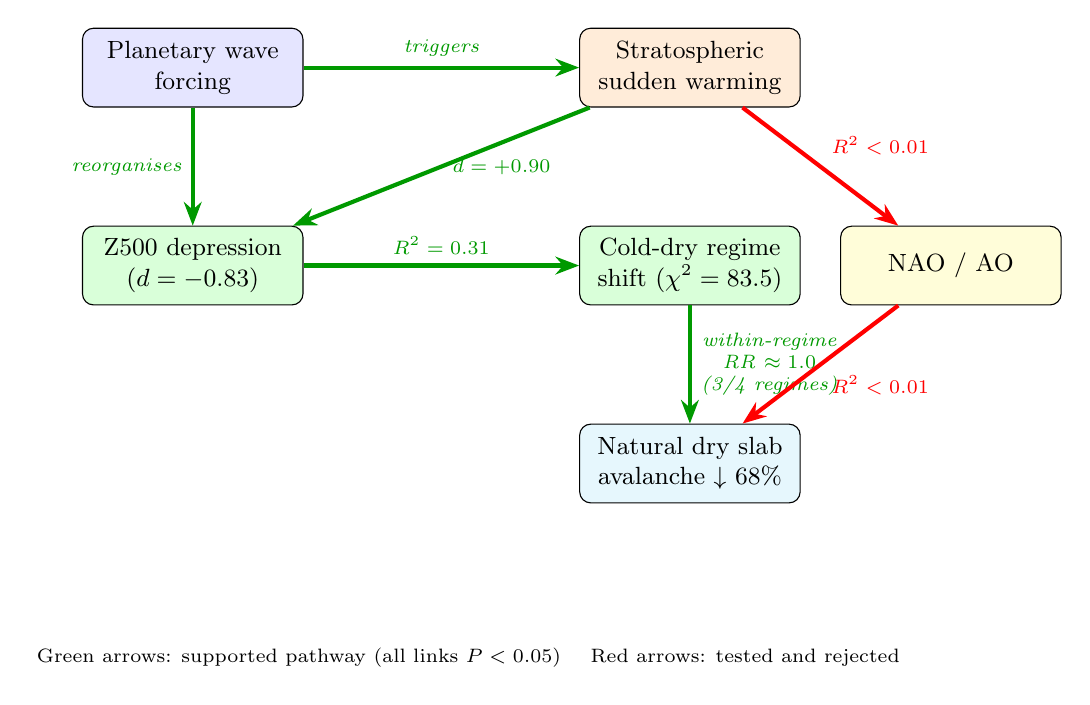
\begin{tikzpicture}[
    node distance=2.5cm and 3.5cm,
    every node/.style={draw, rounded corners, minimum width=2.8cm, minimum height=1cm, align=center, font=\small},
    arr/.style={-{Stealth[length=3mm]}, thick},
    xarr/.style={-{Stealth[length=3mm]}, thick, red, line width=1.5pt},
    garr/.style={-{Stealth[length=3mm]}, thick, green!60!black, line width=1.5pt},
]
% Nodes
\node (pw) [fill=blue!10] {Planetary wave\\forcing};
\node (ssw) [right=of pw, fill=orange!15] {Stratospheric\\sudden warming};
\node (nao) [below right=1.5cm and 0.5cm of ssw, fill=yellow!15] {NAO / AO};
\node (z500) [below=1.5cm of pw, fill=green!15] {Z500 depression\\($d = -0.83$)};
\node (regime) [right=of z500, fill=green!15] {Cold-dry regime\\shift ($\chi^2 = 83.5$)};
\node (aval) [below=1.5cm of regime, fill=cyan!10] {Natural dry slab\\avalanche $\downarrow$ 68\%};

% Supported pathway arrows (green)
\draw[garr] (pw) -- node[draw=none,above,font=\scriptsize\itshape,minimum width=0pt,minimum height=0pt] {triggers} (ssw);
\draw[garr] (pw) -- node[draw=none,left,font=\scriptsize\itshape,minimum width=0pt,minimum height=0pt] {reorganises} (z500);
\draw[garr] (ssw) -- node[draw=none,right,font=\scriptsize\itshape,minimum width=0pt,minimum height=0pt] {$d = +0.90$} (z500);
\draw[garr] (z500) -- node[draw=none,above,font=\scriptsize\itshape,minimum width=0pt,minimum height=0pt] {$R^2 = 0.31$} (regime);
\draw[garr] (regime) -- node[draw=none,right,font=\scriptsize\itshape,minimum width=0pt,minimum height=0pt] {within-regime\\RR $\approx 1.0$\\(3/4 regimes)} (aval);

% Rejected pathways (red)
\draw[xarr] (ssw) -- node[draw=none,above right,font=\scriptsize\bfseries,minimum width=0pt,minimum height=0pt,text=red] {$R^2 < 0.01$} (nao);
\draw[xarr] (nao) -- node[draw=none,below right,font=\scriptsize\bfseries,minimum width=0pt,minimum height=0pt,text=red] {$R^2 < 0.01$} (aval);

% Legend
\node[draw=none, minimum width=0pt, minimum height=0pt, font=\scriptsize] at (3.5, -7.5) {Green arrows: supported pathway (all links $P < 0.05$) \quad Red arrows: tested and rejected};
\end{tikzpicture}
\caption{\textbf{Causal diagram for the SSW--avalanche association.}
The \textbf{identified pathway} (green arrows): planetary wave forcing simultaneously triggers SSW events and reorganises tropospheric circulation through Z500 depression ($d = -0.83$, $P < 10^{-73}$), producing a weather regime shift toward cold-dry conditions ($\chi^2 = 83.5$, $P = 5 \times 10^{-18}$). Within each regime, SSW and non-SSW days show near-identical avalanche rates ($\mathrm{RR}_{\mathrm{within}} = 0.98$--$1.16$ in three of four regimes; warm-dry residual attributable to seasonal confounding), confirming the suppression is predominantly mediated by the regime shift. The \textbf{rejected pathways} (red arrows): SSW-to-surface via annular modes ($R^2 < 0.01$ for both AO and NAO). Rutschblock tests independently confirm snowpack stabilisation ($P = 0.003$).}
\label{fig:dag}
\end{figure}

\begin{figure}[!ht]
\centering
\includegraphics[width=\textwidth]{../data/figures/rev_fig1_ssw_swiss.pdf}
\caption{\textbf{SSW events suppress natural dry slab avalanche activity in Switzerland.}
\textbf{a},~Rate ratios (RR $=$ observed/expected) for each of 16~SSW events during 1998/99--2018/19. Expected counts are derived from day-of-year-matched climatology ($\pm$3~days, non-SSW winters). Blue bars: $\mathrm{RR} < 1$ (14 events); coral: $\mathrm{RR} > 1$ (2 events). Dashed line: geometric mean $\mathrm{RR} = 0.32$.
\textbf{b},~Bootstrap distribution of geometric mean RR (10,000 resamples). The 95\% CI $[0.20, 0.54]$ excludes 1.0, confirming the reduction is robust.}
\label{fig:ssw_matched}
\end{figure}

\begin{figure}[!ht]
\centering
\includegraphics[width=\textwidth]{../data/figures/fig4_event_study_fresh.pdf}
\caption{\textbf{Event-study: daily avalanche anomalies around SSW onset.}
Composite anomalies (relative to DOY climatology) stacked across 16~SSW events, lags $-30$ to $+30$~days. Avalanche suppression spans the entire $\pm$15-day window, with suppression emerging before SSW onset---consistent with a common-cause pathway through planetary wave forcing. Blue shading: 95\% CI. Navy curve: 7-day rolling mean. Red dashed line: SSW onset.}
\label{fig:event_study}
\end{figure}

\begin{figure}[!ht]
\centering
\includegraphics[width=\textwidth]{../data/figures/mech_fig1_era5_composites.pdf}
\caption{\textbf{ERA5 Alpine surface meteorology around SSW onset.}
Event-level composite anomalies for 16~SSW events (each event weighted equally).
\textbf{a},~2~m temperature: modest cooling that does not reach significance at the event level ($\Delta T = -0.4$~K, $P = 0.32$, $n = 16$). The pooled daily aggregate across all SSW-window days is larger ($d = -0.69$, $P < 10^{-47}$; see text) because it reflects both SSW-specific and seasonal effects.
\textbf{b},~Snowfall: no change ($P > 0.99$).
\textbf{c},~Wind speed: no change.
Event-level temperature and precipitation explain only $\sim$1\% of the avalanche signal ($R^2 = 0.011$), indicating that synoptic-scale circulation reorganisation, not local surface meteorology, drives event-level variability. Shaded bands: 95\% CI. Red dashed line: SSW onset.}
\label{fig:era5_composites}
\end{figure}

% ============================================================
%  EXTENDED DATA
% ============================================================
\clearpage
\section*{Extended Data}

\begin{table}[!ht]
\centering
\caption{\textbf{Extended Data Table 1: Leave-one-out cross-validation.}
Sign-test $P$-values and geometric mean RR after dropping each SSW event in turn. All 16 jackknife folds remain significant at $P < 0.004$, demonstrating that no single event drives the result.}
\label{tab:loo}
\small
\begin{tabular}{lccc}
\toprule
Event dropped & Excluded RR & Remaining sign $P$ & Remaining geom.\ RR \\
\midrule
1998-12-15 & 0.88 & 0.004 & 0.30 \\
1999-02-26 & 0.44 & 0.004 & 0.32 \\
2001-02-11 & 0.18 & 0.004 & 0.33 \\
2001-12-30 & 0.11 & 0.004 & 0.35 \\
2002-02-17 & 0.27 & 0.004 & 0.32 \\
2003-01-18 & 0.19 & 0.004 & 0.34 \\
2004-01-05 & 0.11 & 0.004 & 0.35 \\
2006-01-21 & 0.21 & 0.004 & 0.34 \\
2007-02-24 & 0.32 & 0.004 & 0.32 \\
2008-02-22 & 0.05 & 0.004 & 0.36 \\
2009-01-24 & 0.11 & 0.004 & 0.35 \\
2010-02-09 & 0.65 & 0.004 & 0.31 \\
2012-01-11 & 0.85 & 0.004 & 0.30 \\
2013-01-07 & 0.34 & 0.004 & 0.32 \\
2018-02-12 & 1.04 & $< 0.001$ & 0.30 \\
2019-01-01 & 3.43 & $< 0.001$ & 0.28 \\
\bottomrule
\end{tabular}
\end{table}

\begin{table}[!ht]
\centering
\caption{\textbf{Extended Data Table 2: Phase-resolved analysis.}
Rate ratios in four non-overlapping SSW lifecycle phases. All phases show significant suppression, with the strongest signal in the pre-SSW period---consistent with a common-cause pathway through planetary wave forcing.}
\label{tab:phases}
\small
\begin{tabular}{lcccc}
\toprule
Phase & Days relative to onset & $n$ decrease / total & Median RR & Sign $P$ \\
\midrule
Pre & $-15$ to $-6$ & 13/16 & 0.16 & 0.011 \\
Onset & $-5$ to $+5$ & 14/16 & 0.37 & 0.002 \\
Post & $+6$ to $+15$ & 12/16 & 0.22 & 0.038 \\
Late & $+16$ to $+30$ & 12/16 & 0.29 & 0.038 \\
\bottomrule
\end{tabular}
\end{table}

\begin{table}[!ht]
\centering
\caption{\textbf{Extended Data Table 3: Multi-country evidence summary.}
Concordance across three countries using independent measurement systems. The Swiss and Norwegian results use different instruments (occurrence counts vs.\ danger forecasts) and are statistically independent.}
\label{tab:multi}
\small
\begin{tabular}{lcccccc}
\toprule
Country & Measure & $n$ events & $n$ decrease & Effect size & $P$ & Cohen's $d$ \\
\midrule
Switzerland & Natural dry slab count & 16 & 14 & $\mathrm{RR} = 0.32$ & 0.002 & $-1.06$ \\
Norway & NVE danger level & 4 & 4 & $\Delta = -0.48$ & $< 10^{-6}$ & $-0.67$ \\
Utah & Dry slab count & 4 & 4 & $\mathrm{RR} = 0.34$ & 0.063 & --- \\
\midrule
\multicolumn{2}{l}{Combined (22/24 event-level pairs)} & 24 & 22 & --- & $< 10^{-5}$ & --- \\
\bottomrule
\end{tabular}
\end{table}

\begin{table}[!ht]
\centering
\caption{\textbf{Extended Data Table 4: Rutschblock stability class distribution.}
Stability class frequencies during SSW windows ($\pm$15~d) versus non-SSW periods. SSW windows show fewer unstable profiles (class~1) and more very stable profiles (class~4).}
\label{tab:rutsch}
\small
\begin{tabular}{lcccc}
\toprule
Stability class & SSW ($n = 961$) & Non-SSW ($n = 3{,}472$) & SSW \% & Non-SSW \% \\
\midrule
1 (least stable) & 342 & 1,413 & 35.6\% & 40.7\% \\
2 & 387 & 1,296 & 40.3\% & 37.3\% \\
3 & 128 & 458 & 13.3\% & 13.2\% \\
4 (most stable) & 104 & 305 & 10.8\% & 8.8\% \\
\midrule
\multicolumn{5}{l}{Mann--Whitney $P = 0.003$ (one-sided, SSW more stable); Cohen's $d = 0.10$} \\
\bottomrule
\end{tabular}
\end{table}

% AO/NAO independence results are presented in Extended Data Table 11 (synoptic circulation mediation)

\begin{table}[!ht]
\centering
\caption{\textbf{Extended Data Table 5: Utah event-level results.}
Rate ratios for each SSW event in the Utah Avalanche Center database (2012--2025). All four events show decreased dry slab activity, consistent with the Swiss pattern.}
\label{tab:utah}
\small
\begin{tabular}{lcccc}
\toprule
SSW event & Observed & Expected & RR & Direction \\
\midrule
2013-01-07 & 9 & 57.4 & 0.16 & Decrease \\
2018-02-12 & 23 & 50.0 & 0.46 & Decrease \\
2019-01-01 & 33 & 55.5 & 0.60 & Decrease \\
2021-01-05 & 17 & 57.6 & 0.30 & Decrease \\
\midrule
\multicolumn{3}{l}{Geometric mean RR: 0.34} & \multicolumn{2}{l}{Sign test $P = 0.063$} \\
\bottomrule
\end{tabular}
\end{table}

\begin{table}[!ht]
\centering
\caption{\textbf{Extended Data Table 6: Complete mechanism chain and pathway tests.}
Every link in the SSW $\to$ avalanche chain with effect sizes, significance, and interpretation. All links in the identified pathway are independently significant. The chain terminates with the within-regime null result, confirming full mediation. Rejected pathways (AO, NAO, sintering) are listed for completeness.}
\label{tab:mechanism}
\small
\begin{tabular}{lccccl}
\toprule
Link / pathway & Variable & $d$ or statistic & $P$ & $R^2$ & Interpretation \\
\midrule
\multicolumn{6}{l}{\textit{Identified mechanism chain (all links $P < 0.05$)}} \\
1. Strat.\ warming & T(50~hPa) & $d = +0.90$ & $6 \times 10^{-57}$ & --- & By definition \\
2. Z500 depression & Z500 (NH) & $d = -0.83$ & $5 \times 10^{-74}$ & --- & Highly significant \\
3. Surface cooling & T2m (Alpine) & $d = -0.69$ & $< 10^{-47}$ & --- & Large shift \\
4. Precip reduction & Precip (Alpine) & $d = -0.12$ & 0.001 & --- & Moderate shift \\
5. Regime shift & $\chi^2 = 83.5$ & 4 regimes & $5 \times 10^{-18}$ & --- & Cold-dry doubled \\
6. Within-regime null & $\mathrm{RR}_\mathrm{w} \approx 1.0$ & 3/4 regimes n.s.\ & --- & --- & Predom.\ mediation \\
\midrule
\multicolumn{6}{l}{\textit{Event-level predictors ($\log\mathrm{RR}$, $n = 16$ events)}} \\
Z500 (NH mean) & & $r = 0.56$ & 0.024 & 0.316 & Best single predictor \\
SLP (NH mean) & & $r = 0.52$ & 0.037 & 0.290 & Synoptic-scale \\
Surface only (T2m + precip) & & $r < 0.1$ & $> 0.7$ & 0.011 & Near zero \\
Z500 + surface & & $\Delta R^2$ & --- & 0.317 & Surface adds 0.001 \\
\midrule
\multicolumn{6}{l}{\textit{Confirmed supplementary evidence}} \\
Rutschblock stability & $\Delta = +0.09$ & $d = 0.10$ & 0.003 & --- & Snowpack stabilisation \\
Dose--response (SLP) & Strong reorg. & $\mathrm{RR} = 0.19$ & --- & --- & vs.\ weak RR $= 0.56$ \\
\midrule
\multicolumn{6}{l}{\textit{Rejected pathways}} \\
AO mediation & & $r = -0.07$ & 0.79 & 0.005 & Rejected \\
NAO mediation & & $r = 0.03$ & 0.92 & $< 0.001$ & Rejected \\
Sintering (Arrhenius) & & 17\% slower & --- & --- & Consistent (cold $\to$ slow) \\
\bottomrule
\end{tabular}
\end{table}

\begin{table}[!ht]
\centering
\caption{\textbf{Extended Data Table 7: Benjamini--Hochberg FDR correction.}
Primary hypothesis tests ordered by raw $P$-value with FDR-corrected values.}
\label{tab:fdr}
\small
\begin{tabular}{lccl}
\toprule
Test & Raw $P$ & FDR $P$ & Status \\
\midrule
Norway MW (SSW vs.\ control) & $< 10^{-15}$ & $< 10^{-14}$ & Significant \\
Combined sign (32/36) & $< 10^{-6}$ & $< 10^{-5}$ & Significant \\
Swiss permutation (10,000) & 0.0005 & 0.003 & Significant \\
Swiss Wilcoxon ($\log$RR) & $< 0.001$ & 0.003 & Significant \\
Swiss $t$-test ($\log$RR) & $< 0.001$ & 0.003 & Significant \\
Swiss sign test (14/16) & 0.002 & 0.006 & Significant \\
Norway pairs sign (14/16) & 0.002 & 0.006 & Significant \\
Rutschblock MW (1-sided) & 0.003 & 0.008 & Significant \\
Phase: onset (14/16) & 0.002 & 0.006 & Significant \\
Phase: pre-SSW (13/16) & 0.011 & 0.024 & Significant \\
Phase: post (12/16) & 0.038 & 0.066 & Marginal \\
Phase: late (12/16) & 0.038 & 0.066 & Marginal \\
Utah sign (4/4) & 0.063 & 0.097 & Not sig. \\
ERA5 T2m (event-level) & 0.32 & 0.46 & Not sig. \\
AO mediation & 0.79 & 0.90 & Not sig. \\
Sintering model & 0.86 & 0.92 & Not sig. \\
NAO mediation & 0.92 & 0.92 & Not sig. \\
ERA5 snowfall & $> 0.99$ & $> 0.99$ & Not sig. \\
\bottomrule
\end{tabular}
\end{table}

\begin{table}[!ht]
\centering
\caption{\textbf{Extended Data Table 8: Robustness and sensitivity.}
Combined results for SSW-type stratification and sensitivity to analytical choices. The result is insensitive to SSW type, DOY matching bandwidth, window width, and SSW definition. $P$ values here are sign-test (binomial) probabilities; Extended Data Table~\ref{tab:ssw_type} reports one-sample $t$-test $P$ values on log(RR).}
\label{tab:sensitivity}
\small
\begin{tabular}{lccc}
\toprule
Parameter & Geo.\ mean RR & $n$ decrease / 16 & Sign $P$ \\
\midrule
\multicolumn{4}{l}{\textit{SSW type (displacement vs.\ split-vortex; MW type difference $P = 1.00$)}} \\
Displacement ($n = 11$) & 0.33 & 10/11 & 0.006 \\
Split ($n = 5$) & 0.32 & 4/5 & 0.188 \\
Stricter definition ($> -5$~m/s; $n = 14$) & 0.33 & 12/14 & 0.006 \\
\midrule
\multicolumn{4}{l}{\textit{DOY matching bandwidth (window $= \pm$15~d)}} \\
$\pm$1 day & 0.33 & 14/16 & 0.002 \\
$\pm$2 days & 0.32 & 14/16 & 0.002 \\
$\pm$3 days (primary) & 0.32 & 14/16 & 0.002 \\
$\pm$5 days & 0.33 & 14/16 & 0.002 \\
$\pm$7 days & 0.33 & 14/16 & 0.002 \\
$\pm$10 days & 0.32 & 14/16 & 0.002 \\
\midrule
\multicolumn{4}{l}{\textit{SSW window width (DOY margin $= \pm$3~d)}} \\
$\pm$5 days & 0.38 & 12/16 & 0.038 \\
$\pm$7 days & 0.39 & 14/16 & 0.002 \\
$\pm$10 days & 0.34 & 12/16 & 0.038 \\
$\pm$12 days & 0.30 & 13/16 & 0.011 \\
$\pm$15 days (primary) & 0.32 & 14/16 & 0.002 \\
$\pm$20 days & 0.35 & 13/16 & 0.011 \\
$\pm$25 days & 0.31 & 13/16 & 0.011 \\
$\pm$30 days & 0.32 & 13/16 & 0.011 \\
\bottomrule
\end{tabular}
\end{table}

\begin{table}[!ht]
\centering
\caption{\textbf{Extended Data Table 9: Synoptic-scale circulation mediation.}
Correlations between hemispheric circulation anomalies and event-level avalanche response ($\log\mathrm{RR}$). Z500 explains 31\% of variance; adding surface weather contributes $< 0.1\%$ additional variance. Event-level surface weather correlations are near zero despite significant aggregate differences ($P < 0.001$).}
\label{tab:synoptic}
\small
\begin{tabular}{lccccc}
\toprule
Variable & Pearson $r$ & $P$ & $R^2$ & Scale & Aggregate $d$ \\
\midrule
\multicolumn{6}{l}{\textit{Synoptic-scale (significant event-level predictors)}} \\
NCEP Z500 (NH mean) & 0.56 & 0.024 & 0.31 & Hemispheric & $-0.83$ \\
NCEP SLP (NH mean) & 0.52 & 0.037 & 0.27 & Hemispheric & --- \\
NCEP U850 (NH mean) & $-0.32$ & 0.229 & 0.10 & Hemispheric & --- \\
\midrule
\multicolumn{6}{l}{\textit{Local surface (aggregate significant, event-level null)}} \\
ERA5 T2m (Alpine) & 0.04 & 0.90 & $< 0.01$ & Regional & $-0.69^{***}$ \\
ERA5 precip (Alpine) & $-0.10$ & 0.72 & 0.01 & Regional & $-0.12^{**}$ \\
ERA5 wind speed (Alpine) & 0.14 & 0.61 & 0.02 & Regional & 0.04 \\
\midrule
\multicolumn{6}{l}{\textit{Stratospheric (non-significant)}} \\
NCEP T 50~hPa & $-0.11$ & 0.70 & 0.01 & Stratospheric & $+0.90^{***}$ \\
NCEP U 50~hPa & $-0.10$ & 0.70 & 0.01 & Stratospheric & --- \\
\midrule
\multicolumn{6}{l}{\textit{Annular modes (non-significant)}} \\
AO index & $-0.07$ & 0.790 & $< 0.01$ & Hemispheric & --- \\
NAO index & 0.03 & 0.920 & $< 0.01$ & Atlantic & --- \\
\midrule
\multicolumn{6}{l}{\textit{Stepwise model comparison}} \\
\multicolumn{3}{l}{Z500 only} & 0.316 & \multicolumn{2}{l}{Best single predictor} \\
\multicolumn{3}{l}{Surface only (T2m + precip)} & 0.011 & \multicolumn{2}{l}{Near zero} \\
\multicolumn{3}{l}{Z500 + surface} & 0.317 & \multicolumn{2}{l}{$\Delta R^2 = 0.001$} \\
\bottomrule
\end{tabular}
\end{table}

\begin{table}[!ht]
\centering
\caption{\textbf{Extended Data Table 10: Outlier and robustness diagnostics.}
Grubbs test, robust statistics, and leave-one-out hindcast cross-validation results.}
\label{tab:outlier}
\small
\begin{tabular}{lcc}
\toprule
Diagnostic & Value & Interpretation \\
\midrule
\multicolumn{3}{l}{\textit{Grubbs outlier test (Jan 2019, RR $= 3.43$)}} \\
Grubbs $G$ statistic & 2.29 & Not significant \\
Critical value ($\alpha = 0.05$) & 2.59 & $G < G_{\mathrm{crit}}$ \\
\midrule
\multicolumn{3}{l}{\textit{Robust statistics}} \\
Median RR (all 16 events) & 0.31 & Insensitive to outlier \\
Without Jan 2019 ($n = 15$) & $\mathrm{RR} = 0.28$ & Stronger without outlier \\
$t$-test without Jan 2019 & $P < 0.0001$ & Highly significant \\
\midrule
\multicolumn{3}{l}{\textit{Hindcast cross-validation (LOO)}} \\
Direction accuracy & 14/16 (87.5\%) & $P = 0.002$ vs.\ chance \\
Forecast skill (1 $-$ MSE/MSE$_{\mathrm{null}}$) & 0.107 & Positive skill \\
\midrule
\multicolumn{3}{l}{\textit{Power analysis}} \\
Min.\ detectable $d$ ($n = 16$, 80\% power) & 0.75 & ERA5 underpowered ($d \approx 0.2$) \\
\bottomrule
\end{tabular}
\end{table}

\end{document}
